%=======================================================================
%  Sensor-Aware Hypothesis Bank for Passive Frequency-Hopping
%  Generator Identification, Prediction and Response
%  IEEE conference paper (IEEEtran, two-column). Target: <= 6 pages.
%  Figures in figures/, numbers from results/ and docs/paper/ieee/data/.
%=======================================================================
\documentclass[conference]{IEEEtran}
\IEEEoverridecommandlockouts
\usepackage{cite}
\usepackage{amsmath,amssymb,amsfonts}
\usepackage{algorithm}
\usepackage{algorithmic}
\usepackage{graphicx}
\usepackage{textcomp}
\usepackage{booktabs}
\usepackage{multirow}
\usepackage{xcolor}
\usepackage{array}
\usepackage{stfloats}
\graphicspath{{figures/}}
\def\BibTeX{{\rm B\kern-.05em{\sc i\kern-.025em b}\kern-.08em
    T\kern-.1667em\lower.7ex\hbox{E}\kern-.125emX}}

\begin{document}

\title{A Sensor-Aware Hypothesis Bank for Passive Frequency-Hopping
Generator Identification, Next-Channel Prediction and Calibrated Response}

\author{\IEEEauthorblockN{Ehsan Samir}
\IEEEauthorblockA{\textit{Dept. of Electrical and Computer Engineering} \\
\textit{Institution Name}\\
City, Country \\
author@institution.edu}
}

\maketitle

\begin{abstract}
A passive electronic-support receiver that watches a frequency-hopping (FH)
emitter must decide, inside a short engagement window and through a lossy
sensor, which generator drives the hop sequence, what channel comes next, and
whether the stream is predictable at all. We present OTS, a software system
that scores a heterogeneous bank of generator hypotheses---shift registers,
congruential and weak-seed generators, chaotic maps, a Markov hopper, and an
explicit generative none-of-the-above class---through one shared
detection-level likelihood parameterised by the sensor's detection and
false-alarm probabilities. The same likelihood drives anytime-valid stopping,
a training-free next-channel predictor that keeps working on generators the
bank has no expert for, a change-point tracker that detects and re-identifies a
mid-engagement change of generator, and a conformal prediction set whose size
adapts to give a distribution-free coverage guarantee that transfers directly
to the fraction of hops a multi-tone response denies. Across more than
$15{,}000$ simulated episodes spanning thirteen generators and four sensor
operating points, in-bank families are identified at $\geq 0.99$ accuracy in
4--13 hops, the dangerous error of falsely naming an algebraic generator stays
at or below $0.05$ everywhere, next-channel prediction reaches $1.00$
steady-state top-1 on held-out generators where an identification-only bank
collapses to $0.35$, and conformal sets hold $\geq 0.90$ coverage where a fixed
shortlist covers as little as $0.19$. The measured hops-to-identify sits within
$1.3$--$2.7\times$ an information-theoretic lower bound.
\end{abstract}

\begin{IEEEkeywords}
frequency hopping, electronic support, sequential hypothesis testing,
online prediction, conformal prediction, change-point detection.
\end{IEEEkeywords}

%=======================================================================
\section{Introduction}
%=======================================================================
Frequency hopping (FH) is the standard way a radio link resists interception
and jamming: the carrier moves between channels under a pseudo-random
generator known only to the communicating parties. A passive electronic-support
(ES) receiver that wishes to characterise such an emitter faces three coupled
questions. \emph{Which} generator is in use, so that past hops constrain future
ones? \emph{What} channel will be used next, which is the quantity any response
must act on? And \emph{how predictable} is the emitter at all, since a keyed
cryptographic generator is, by design, indistinguishable from noise and should
be reported as such rather than chased. These questions must be answered inside
an engagement window of tens of hops and through a sensor that misses true
hops and reports phantom ones.

Most prior work answers only one question and assumes a clean stream. Neural
predictors forecast the next hop of a specific family from an idealised
sequence~\cite{li2020lstm,li2021china,zhu2023recovery,basak2024spectrum};
sequential detectors identify a parameter but not a heterogeneous family
set~\cite{baum1994,dragalin1999}; particle filters track a hopped carrier but
not the \emph{algorithm} behind it~\cite{valyrakis2009,sidiropoulos2006}. None
scores a bank of competing generator families through an explicit sensor model,
and none couples a calibrated forecast to a decision with a stated guarantee.

This paper presents OTS, a system built around a single idea: reduce the lossy
sensor to a per-slot \emph{detection-level likelihood} and use that one
quantity everywhere. The contributions, each backed by a simulation
experiment under the information-parity rule that every expert sees only the
sensor's detections, are:
\begin{enumerate}
\item A unified sensor-aware hypothesis bank that scores shift-register,
congruential, weak-seed, chaotic and Markov generators plus an explicit
generative none-of-the-above class $H_0$ through one $(P_d,P_{fa})$ likelihood,
with MSPRT and anytime-valid e-process stopping (Sec.~\ref{sec:bank}).
\item A training-free, online next-channel predictor (a Fixed-Share mixture
carrying a universal context-mixing expert) that keeps predicting on generators
the bank has no expert for, and correctly falls to chance on a cryptographic
generator (Sec.~\ref{sec:predict}).
\item A change-point tracker that detects, dates and re-identifies a
mid-engagement change of the generating algorithm from the lossy passive stream
(Sec.~\ref{sec:switch}).
\item A conformal next-channel set whose size adapts to give a
distribution-free coverage guarantee, which transfers to a
``fraction-of-hops-denied'' guarantee for a multi-tone response
(Sec.~\ref{sec:conformal}).
\end{enumerate}
We evaluate on thirteen generators across four sensor operating points,
report a mis-specified-sensor stress test, and compare the measured
identification cost against an information-theoretic converse.

%=======================================================================
\section{Related Work}
%=======================================================================
\textbf{FH prediction.} Deep models predict FH sequences from time--frequency
representations~\cite{li2020lstm,li2021china,zhu2023recovery,lee2020detection},
including CNN--LSTM drone FHSS occupancy validated on real
signals~\cite{basak2024spectrum}; all are trained per family on clean
spectrograms. The closest precedent to our ``identify, predict, flag unknown''
loop reverse-engineers LFSR hoppers with a neural network~\cite{strickland2023},
but is LFSR-only, trained, and clean-data; transformers predict
linear-congruential outputs in-context~\cite{tao2025transformers}. Our predictor
differs by being training-free, online, scored under detection losses, and tied
to an identification bank.

\textbf{Sequential tests and sensor likelihoods.} Threshold stopping is the
MSPRT of~\cite{baum1994}, optimal under correlation~\cite{dragalin1999}; the
e-process is a safe anytime-valid test~\cite{ramdas2023}; the generative
none-of-the-above class is the no-match idea of~\cite{gutman1989}. The reduced
emission is the discrete-channel detection/clutter likelihood behind
probabilistic data association~\cite{barshalom2009}; particle filters track a
hopped carrier~\cite{valyrakis2009,sidiropoulos2006} but not the algorithm.

\textbf{Change-point, conformal and application.} A run-length posterior
carrying candidate models is the architecture of~\cite{knoblauch2018},
built on~\cite{adams2007}; our set uses Adaptive Conformal
Inference~\cite{gibbs2021} for non-exchangeable streams; recurrence recovery
draws on classical cryptanalysis~\cite{massey1969,reeds1977}. Bluetooth
hop-prediction attacks~\cite{blueear2016} are a deployed intercept-and-act
instance, and learned anti-jamming hopping is the dual
problem~\cite{qi2024drl}; we treat the multi-tone response only as a downstream
use of the calibrated forecast, not a new jammer.

%=======================================================================
\section{System Model and Methodology}
\label{sec:method}
%=======================================================================
Fig.~\ref{fig:arch} shows the end-to-end data flow and Fig.~\ref{fig:method}
the per-slot loop (Algorithm~\ref{alg:loop}).

\begin{figure}[t]
\centering
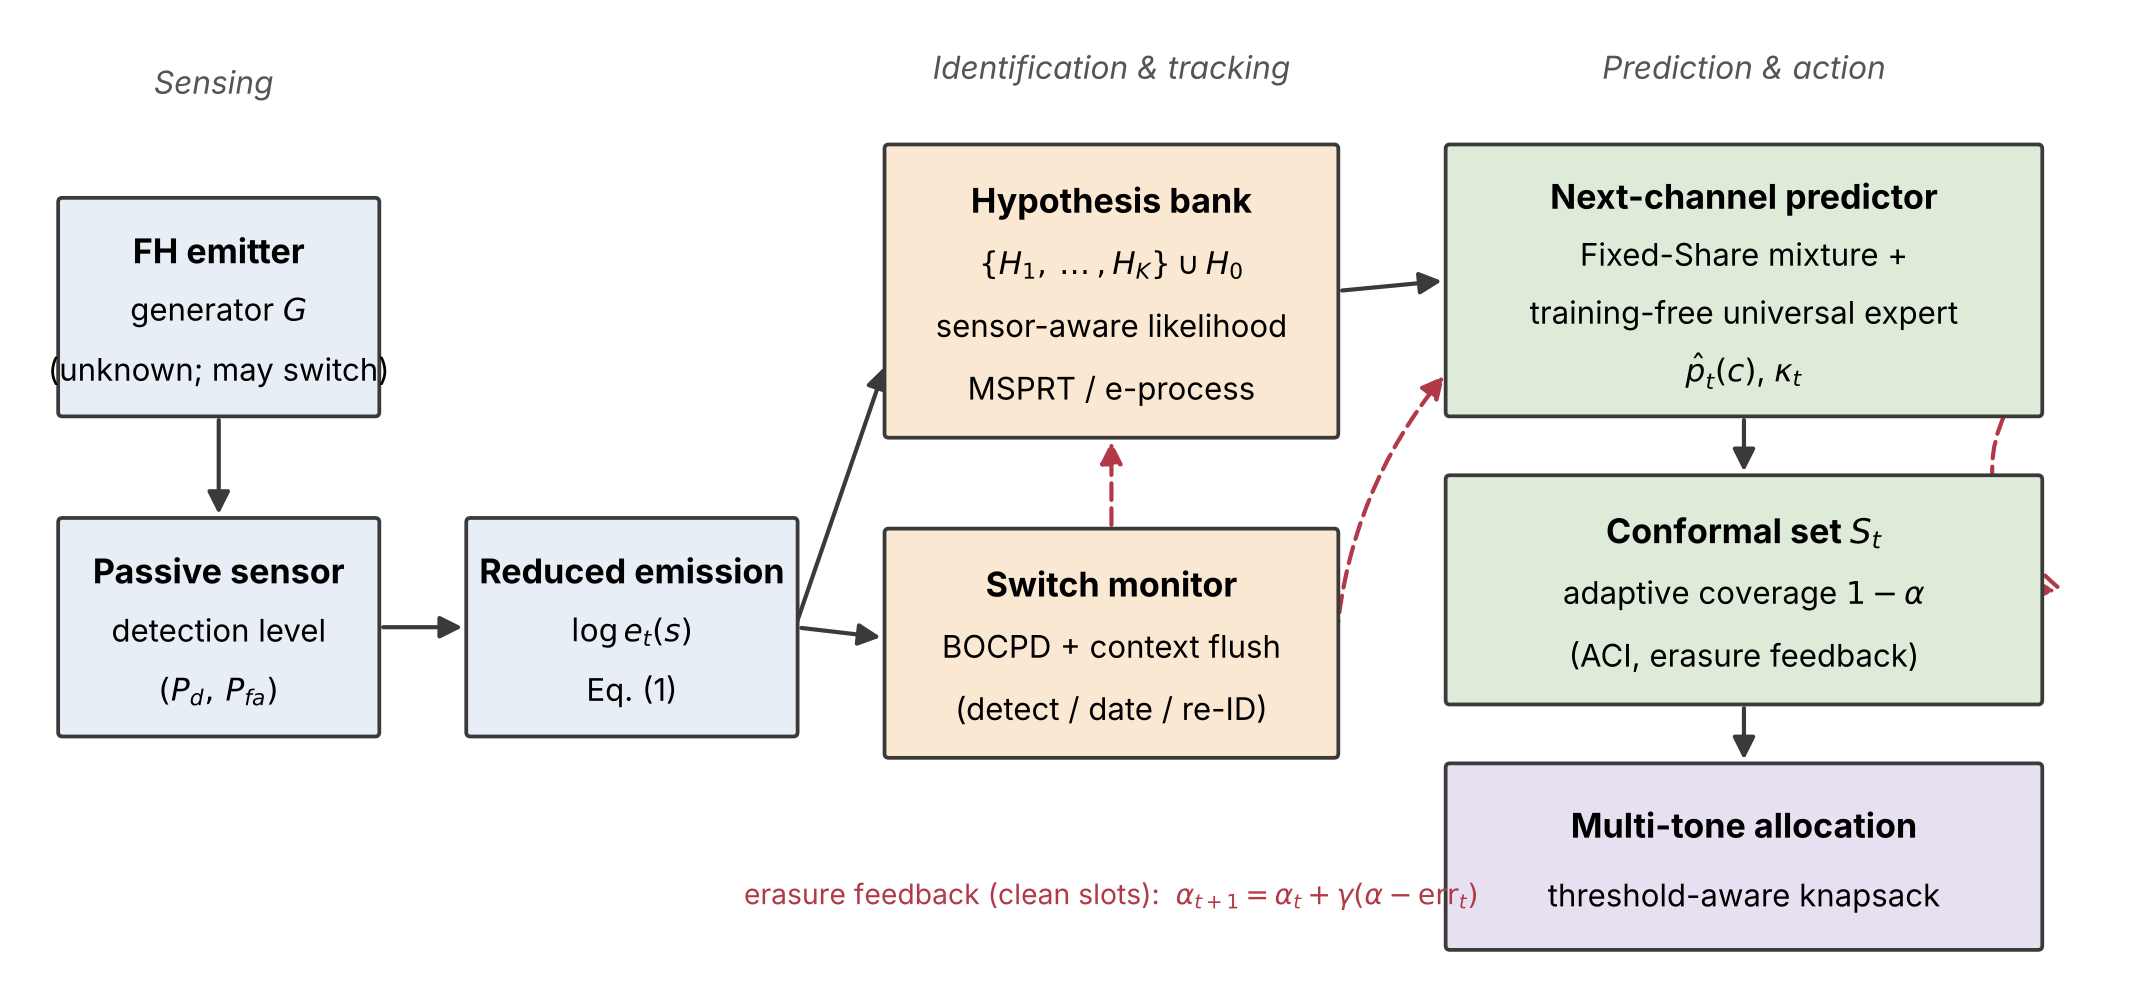
\includegraphics[width=\columnwidth]{fig_architecture.png}
\caption{System architecture. One detection-level likelihood feeds the
hypothesis bank, the switch monitor, the next-channel predictor and the
conformal set; the set drives the multi-tone response. Dashed red: the switch
monitor resets the bank/predictor, and erasure feedback calibrates the
conformal level online.}
\label{fig:arch}
\end{figure}

\subsection{Problem and sensor model}
A single emitter transmits, at slot $t=1,\dots,T$, on channel $c_t$ from a set
$C$ of size $M$ (default $M=16$), chosen by an unknown generator $G$. A passive
sensor detects the true channel with probability $P_d$ and raises an
independent false alarm on every other channel with probability $P_{fa}$,
producing a detection set $D_t\subseteq C$. For a hypothesised true channel $s$,
factoring out the all-false-alarm constant $F_t$ (identical across hypotheses)
leaves the \emph{reduced emission}
\begin{equation}
\log e_t(s)=
\begin{cases}
\log(P_d/P_{fa}), & s\in D_t,\\[2pt]
\log\!\big((1-P_d)/(1-P_{fa})\big), & s\notin D_t.
\end{cases}
\label{eq:emit}
\end{equation}
$F_t$ cancels in every posterior and likelihood ratio, so the whole system
works with \eqref{eq:emit}, which is used twice: once to generate observations
and once inside every expert. Because the same simulator generates adversaries
and scores them, we enforce \emph{information parity}: an expert sees only the
stream of observations and its own bounded reconnaissance ranges, never the true
channel sequence or the generator instance.

\subsection{The hypothesis bank and stopping rules}
\label{sec:bank}
The bank keeps a posterior over $\{H_0,H_1,\dots,H_K\}$ and updates it after
every slot with each expert's reduced likelihood,
$\pi_t(k)\propto\pi_{t-1}(k)\,P(o_t\mid o_{1:t-1},H_k)$, with a floor on the
$H_0$ prior so the unknown class is never ruled out. Deterministic families
(LFSR, filtered LFSR, LCG, weak-seed) are realised by a particle filter over
the family's parameter space: each candidate parameterisation is one particle
whose deterministic trajectory is scored through \eqref{eq:emit}, which is
immune to gaps because it never needs consecutive outputs. Markov and chaotic
families use a channel-level HMM forward pass.

Two stopping rules read the cumulative reduced log-likelihoods. \emph{MSPRT}
declares $k^\ast=\arg\max_k\pi_t(k)$ when $\pi_t(k^\ast)\geq1-\delta$;
$k^\ast=0$ means \emph{unknown}. The \emph{e-process} declares $k$ when the
e-value against its strongest competitor,
$E_t(k)=P(o_{1:t}\mid H_k)/\max_{j\neq k}P(o_{1:t}\mid H_j)$, crosses $1/\beta$;
by Ville's inequality this bounds the probability of ever declaring a wrong
in-bank $k$ by $\beta$ per competitor.

\subsection{Next-channel prediction}
\label{sec:predict}
Identification is a means; the deliverable is the next channel. A Fixed-Share
expert mixture weights experts by their \emph{recent} one-step predictive skill,
\begin{equation}
w_{t+1}(i)\propto w_t(i)\,e^{\eta\,\ell_t(i)},\quad
w_{t+1}\leftarrow(1-\alpha)w_{t+1}+\alpha/N,
\end{equation}
and mixes their forecasts, $\hat p_t(c)=\sum_i w_t(i)\,p_i(c)$. The share floor
$\alpha$ lets a dormant expert recover after a change. Crucially, the mixture
always carries a \emph{training-free universal} expert---a gap-robust
variable-order context-mixing model---so when no identification expert fits a
new generator, the universal expert accrues weight and carries the forecast
instead of collapsing to the uniform floor. The system also reports the
predictability score $\kappa_t=1-H(\hat p_t)/\log M$.

\subsection{Switch tracking}
\label{sec:switch}
A cumulative-evidence identifier is slow to forget. A Bayesian online
change-point posterior whose run-length hypotheses each carry a bank
\emph{anchored at the hypothesised switch slot} lets a freshly re-keyed or
counter-based generator restart at zero, so one posterior detects, dates,
re-identifies and predicts simultaneously. A cheaper CUSUM monitor on the
mixture's loss stream additionally resets the Fixed-Share weights and flushes
the universal predictor's stale context on an alarm.

\begin{figure}[t]
\centering
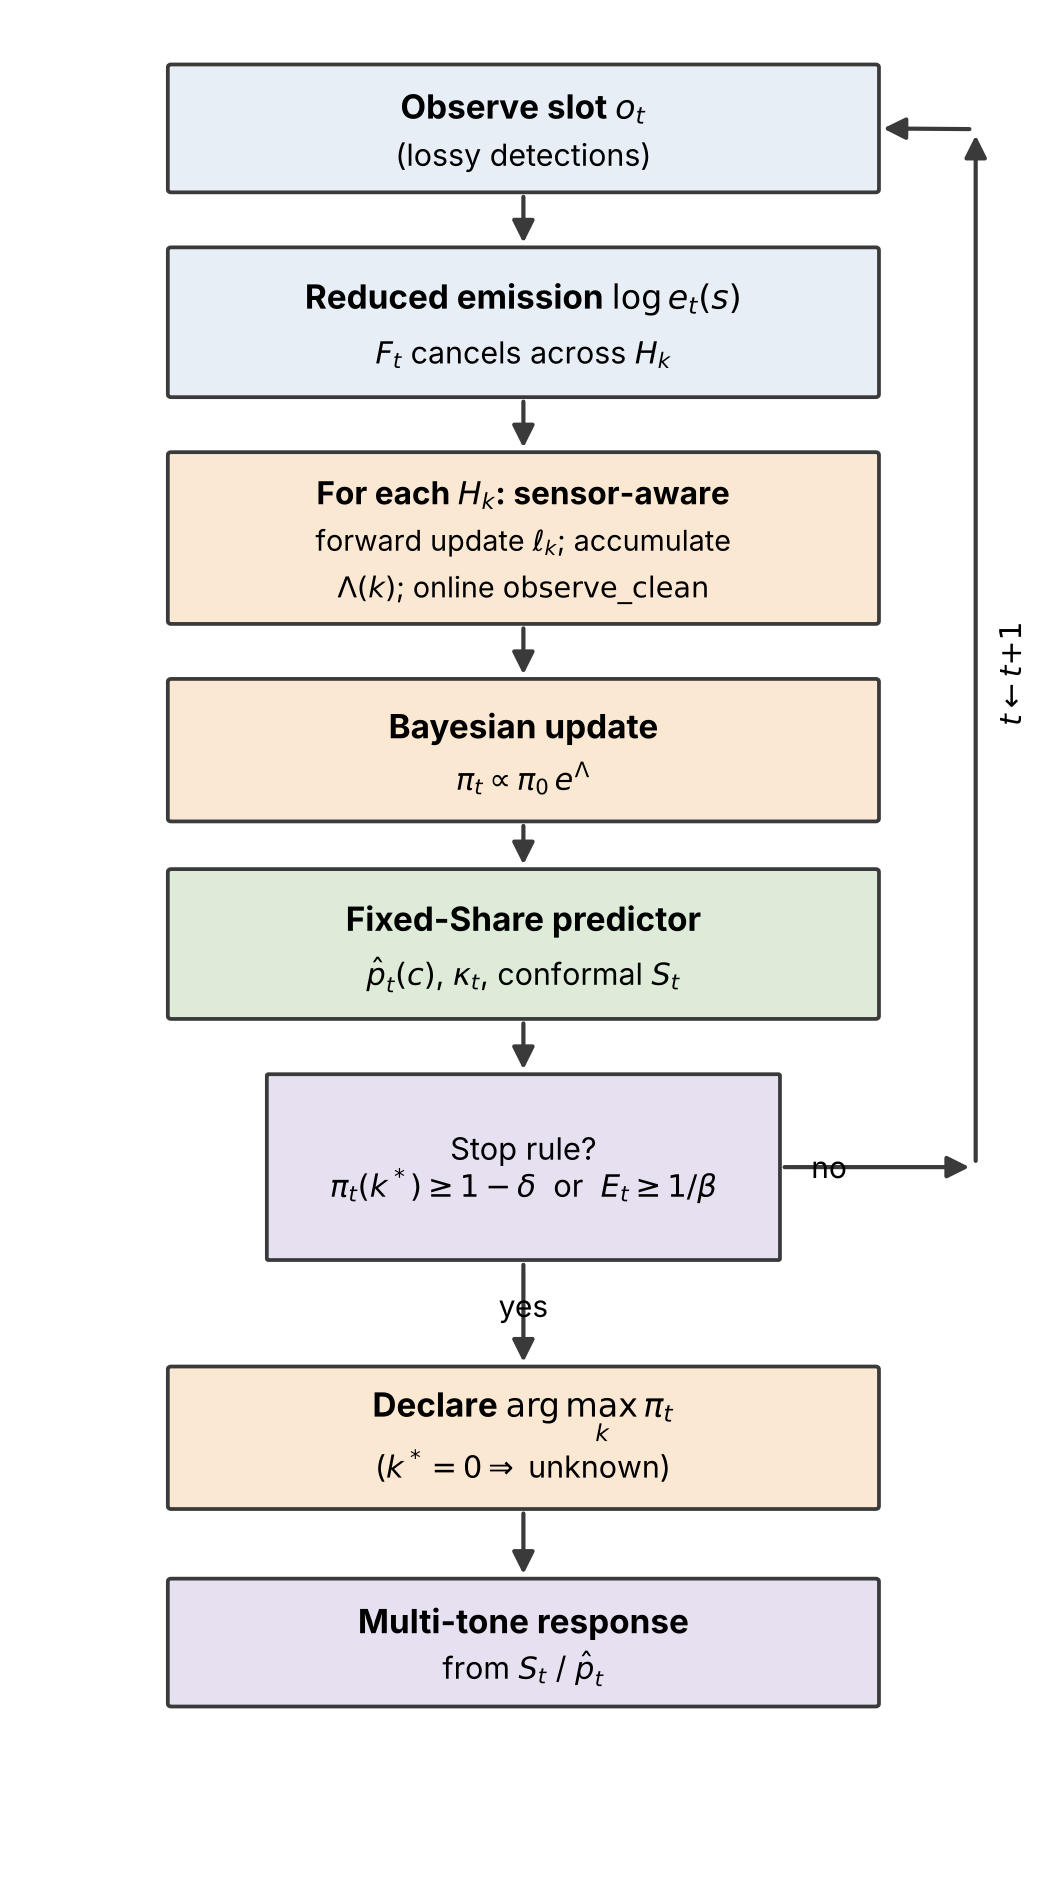
\includegraphics[width=0.84\columnwidth]{fig_methodology.png}
\caption{Per-slot engagement loop (Algorithm~\ref{alg:loop}). One reduced
emission drives the Bayesian update, the Fixed-Share predictor and the stopping
test; the loop runs until a declaration or the window ends.}
\label{fig:method}
\end{figure}

\subsection{Conformal sets and response}
\label{sec:conformal}
A point forecast carries no guarantee. We emit a prediction set $S_t$: the
smallest top-ranked set whose predictive mass reaches an online level
$1-\alpha_t$, with $\alpha_t$ updated by Adaptive Conformal
Inference~\cite{gibbs2021},
$\alpha_{t+1}=\mathrm{clip}(\alpha_t+\gamma(\alpha-\mathrm{err}_t),0,1)$. The
calibration signal $\mathrm{err}_t$ is the erasure feedback a passive node
actually receives (clean slots only), so coverage holds over the clean
sub-stream without assuming exchangeability. Because the set \emph{is} the
multi-tone jam plan, funding every channel in $S_t$ denies the realised next
hop at the coverage rate, so the fraction of hops denied inherits the
distribution-free $1-\alpha$ bound. A threshold-aware greedy knapsack
(rank channels by predicted mass per unit denial cost, fund to a budget) is the
underlying allocator.

\begin{algorithm}[t]
\caption{Engagement loop (one emitter, window $T$)}
\label{alg:loop}
\begin{algorithmic}
\STATE $\pi\leftarrow\pi_0$; reset every expert
\FOR{$t=1$ \TO $T$}
  \STATE $o_t\leftarrow\mathrm{observe}()$; form $\log e_t$ by \eqref{eq:emit}
  \FOR{$k=0$ \TO $K$}
     \STATE $\ell_k\leftarrow H_k.\mathrm{step}(\log e_t)$;\;
            $\Lambda(k)\mathrel{+}=\ell_k$;\; $H_k.\mathrm{observe\_clean}(o_t)$
  \ENDFOR
  \STATE $\pi\leftarrow\mathrm{softmax}(\log\pi_0+\Lambda)$
  \STATE $\hat p\leftarrow$ Fixed-Share predictor; form set $S_t$
  \IF{stop rule fires}
     \STATE \textbf{return} declare$(\arg\max_k\pi)$, $\tau=t$
  \ENDIF
\ENDFOR
\STATE \textbf{return} declare$(\arg\max_k\pi)$, $\tau=T$
\end{algorithmic}
\end{algorithm}

%=======================================================================
\section{Experimental Setup}
\label{sec:setup}
%=======================================================================
All experiments are simulation-only with $M=16$, fixed seeds, and figures
regenerated from saved JSON. Table~\ref{tab:gens} lists the generator library.
Three ``held-out'' families (lagged Fibonacci, quadratic congruential, sine map)
have \emph{no} dedicated expert and test prediction generalisation; a keyed
SHA-256 CSPRNG is the unpredictable control. We sweep four sensor operating
points: Perfect $(1.0,0)$, Strong $(0.95,0.01)$, Typical $(0.8,0.02)$ and
Contested $(0.6,0.05)$. Identification uses MSPRT with $\delta=0.05$. We report
identification accuracy, hops-to-identify $\tau$, and the \emph{hard} false-ID
rate---declaring an algebraic family (LFSR, filtered LFSR, LCG, weak-seed) that
is not the truth, the dangerous error. Prediction is scored by steady-state
top-1 next-channel accuracy against the chance line $1/M=0.0625$. The headline
identification evaluation aggregates $100$ seeds $\times$ $13$ generators
$\times$ $4$ sensors ($5{,}200$ episodes); the coverage experiment adds $7{,}500$.

\begin{table}[t]
\centering
\caption{Generator library. Held-out families have no expert.}
\label{tab:gens}
\setlength{\tabcolsep}{4pt}
\footnotesize
\begin{tabular}{@{}lll@{}}
\toprule
Family & Structure & Hidden parameters \\
\midrule
LFSR / filt.\ LFSR & shift register ($+$ combiner) & taps, length, state \\
LCG / full LCG & $x\!\leftarrow\!(ax{+}c)\bmod m$ & $m,a,c,\text{seed}$ \\
weak-seed & small-keyspace PRNG & seed \\
Markov & first-order hopper & transition matrix \\
logistic/tent/H\'enon & chaotic maps, quantised & map parameter, $x_0$ \\
\midrule
lagged-Fib. (held out) & $c_t{=}(c_{t-1}{+}c_{t-k})\bmod M$ & order $k$ \\
quad.-CG (held out) & $x\!\leftarrow\!(ax^2{+}bx{+}c)\bmod M$ & $a,b,c$ \\
sine map (held out) & $x\!\leftarrow\!r\sin(\pi x)$ & $r,x_0$ \\
CSPRNG (control) & SHA-256 counter mode & key \\
\bottomrule
\end{tabular}
\end{table}

%=======================================================================
\section{Results}
\label{sec:results}
%=======================================================================

\subsection{Identification: coverage and safety}
Fig.~\ref{fig:confusion} shows family confusion matrices at the four sensors.
The diagonal is clean for every generator an expert targets. As the sensor
degrades, errors are \emph{graceful}: a held-out generator or a worn-down
Markov source routes to the Markov or $H_0$ column, never to a false algebraic
claim. Table~\ref{tab:ident} aggregates the identifiable families.
Deterministic families are named at $1.00$ accuracy in a handful of hops even on
the contested sensor; the hard false-ID rate stays at or below $0.05$
throughout, and is $0.00$ for the shift-register and weak-seed families that an
operator would most dangerously misattribute.

\begin{figure*}[t]
\centering
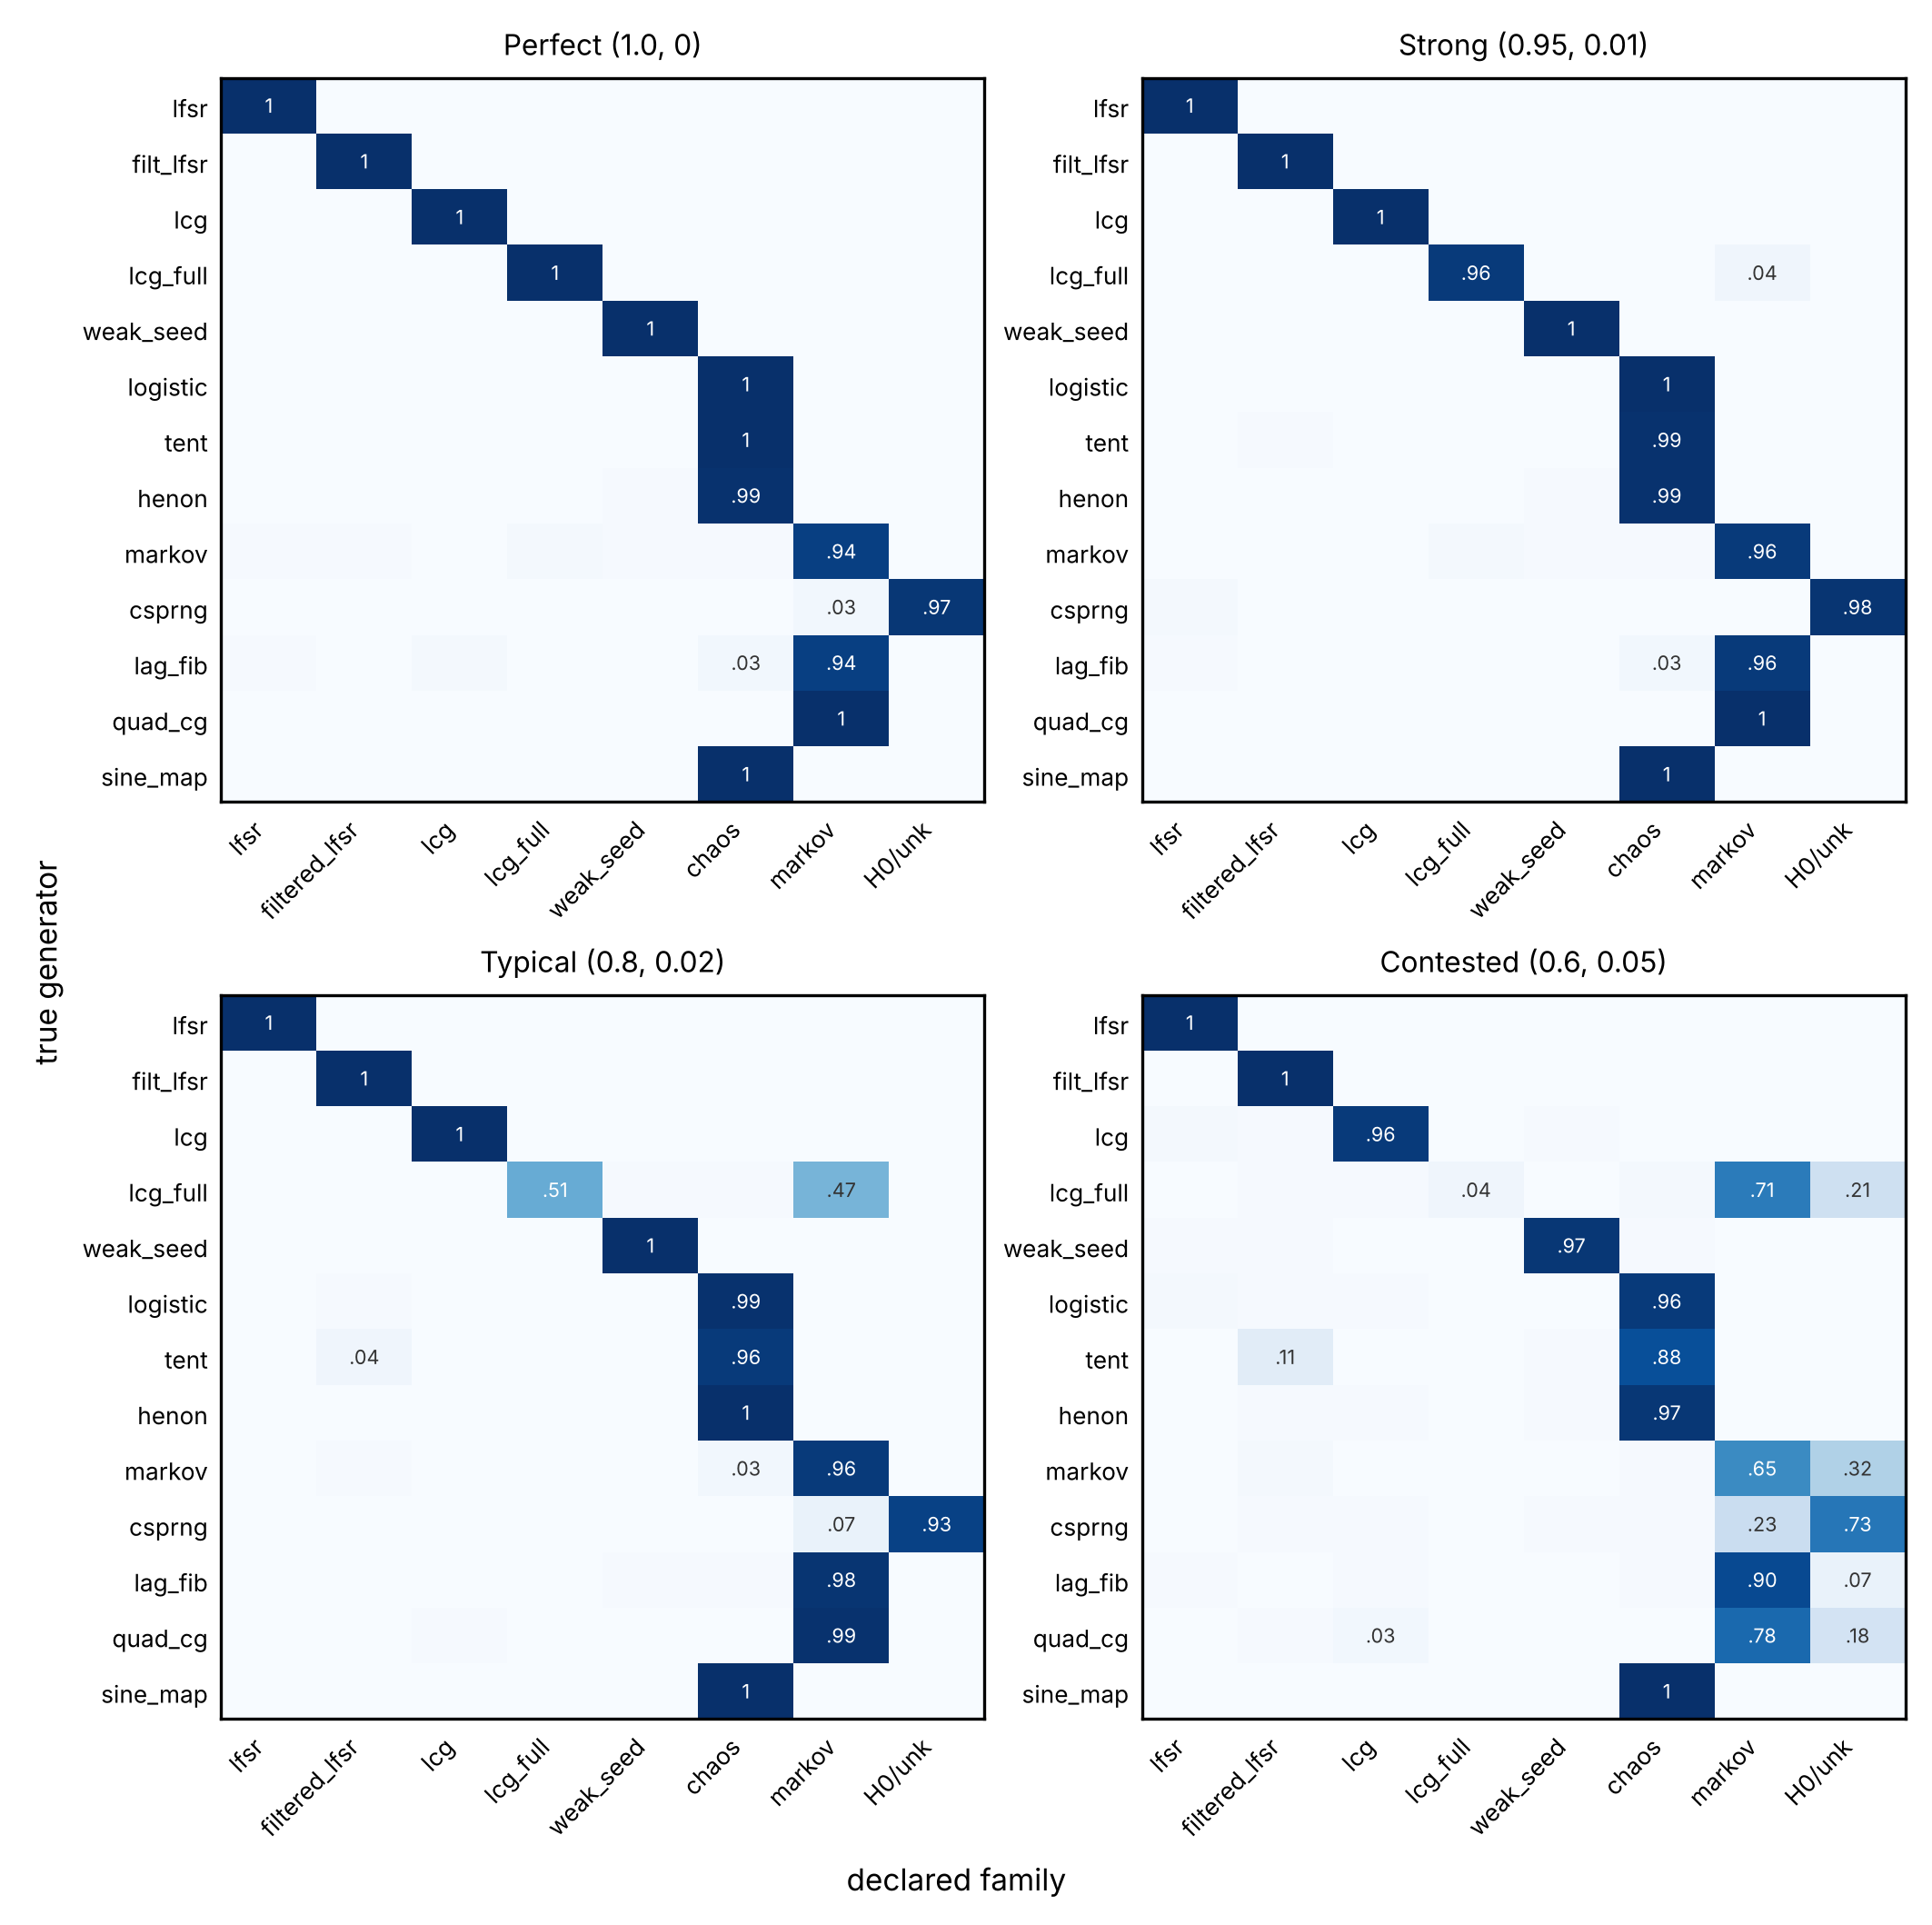
\includegraphics[width=0.92\textwidth]{fig_confusion.png}
\caption{Family confusion matrices (true generator vs declared family), one per
sensor, $100$ seeds per cell. Rows are the thirteen generators including the
three held-out families and the CSPRNG; columns are the declared families and
$H_0$/unknown. The diagonal stays clean for identifiable families; held-out and
unbreakable sources degrade to Markov/$H_0$, never to a false algebraic claim,
even on the contested sensor.}
\label{fig:confusion}
\end{figure*}

\begin{table}[t]
\centering
\caption{Identification accuracy / hard false-ID across sensors (100 seeds).}
\label{tab:ident}
\setlength{\tabcolsep}{3.4pt}
\footnotesize
\begin{tabular}{@{}lcccc@{}}
\toprule
 & Perfect & Strong & Typical & Contested \\
Generator & \multicolumn{4}{c}{accuracy / hard false-ID} \\
\midrule
LFSR         & 1.00 / .00 & 1.00 / .00 & 1.00 / .00 & 1.00 / .00 \\
filt.\ LFSR  & 1.00 / .00 & 1.00 / .00 & 1.00 / .00 & 1.00 / .00 \\
LCG          & 1.00 / .00 & 1.00 / .00 & 1.00 / .00 & 0.96 / .04 \\
weak-seed    & 1.00 / .00 & 1.00 / .00 & 1.00 / .00 & 0.97 / .00 \\
chaos (log.) & 1.00 / .00 & 1.00 / .00 & 0.99 / .00 & 0.96 / .00 \\
Markov       & 0.94 / .05 & 0.96 / .01 & 0.96 / .01 & 0.65 / .02 \\
CSPRNG       & 0.97 / .00 & 0.98 / .00 & 0.93 / .00 & 0.73 / .03 \\
\bottomrule
\end{tabular}
\end{table}

\subsection{The value of the sensor-aware likelihood}
Replacing \eqref{eq:emit} with a naive clean-match score leaves the two in
agreement while detections are plentiful, but as $P_d$ falls to $0.5$
(at $P_{fa}=0.05$) the naive bank drops to $0.60$ accuracy against $0.98$ and
needs $21.1$ hops against $15.3$, because it reads a missed hop as evidence
against the truth and a phantom as evidence for a wrong generator. At the level
of a single recovery algorithm the effect is a cliff: plain Berlekamp--Massey
recovers an $L{=}7$ LFSR on every run at $P_d{=}1$ and on \emph{no} run for any
$P_d<1$, while the state-enumeration recovery under \eqref{eq:emit} holds $1.00$
across the whole sweep---the gap is exactly the value of modelling the sensor
inside the likelihood.

\subsection{Mis-specified sensor}
The bank scores with the same $(P_d,P_{fa})$ that generated the data; a referee
will ask what happens when they differ. Fig.~\ref{fig:mismatch} sweeps the
assumed value against the true one. Identification is strikingly robust to an
over-optimistic $P_d$: accuracy stays high across the off-diagonal, because a
missed hop merely omits a likelihood factor rather than corrupting one, and the
hard false-ID rate under a mis-specified $P_{fa}$ stays low. The system is
sensor-\emph{aware} rather than sensor-\emph{oracle}: it degrades gently rather
than failing when its sensor estimate is wrong.

\begin{figure}[t]
\centering
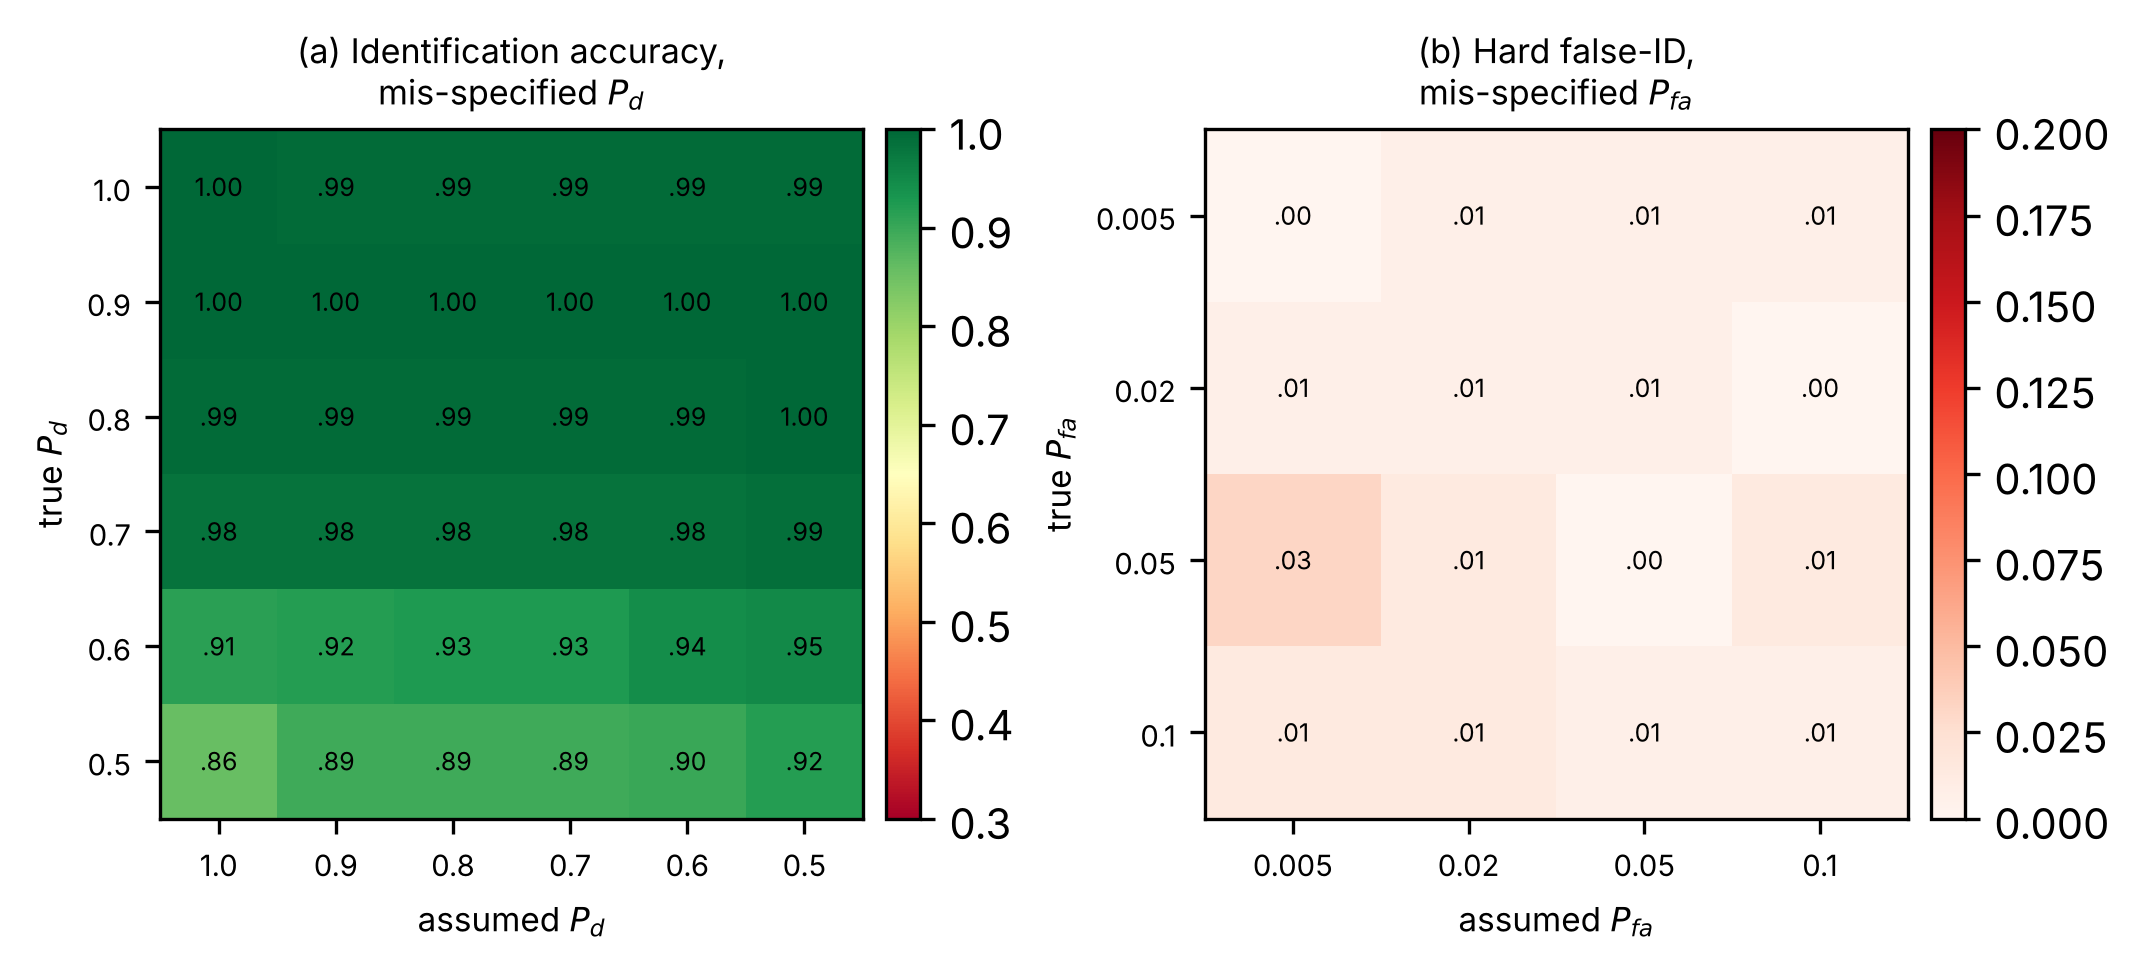
\includegraphics[width=\columnwidth]{fig_mismatch.png}
\caption{Mis-specified sensor. (a) Identification accuracy as the assumed $P_d$
(columns) departs from the true $P_d$ (rows). (b) Hard false-ID as the assumed
$P_{fa}$ departs from the true $P_{fa}$. Accuracy and safety hold across a wide
mismatch band.}
\label{fig:mismatch}
\end{figure}

\subsection{Next-channel prediction and conformal sets}
Fig.~\ref{fig:results} collects the headline prediction results.
Panel~(b) is the central claim: on the held-out lagged-Fibonacci generator the
proposed predictor reaches $1.00$ steady-state top-1 while an
identification-only bank manages $0.35$, because the universal context-mixing
expert recovers the order-2 rule that no bank expert can represent. On a keyed
CSPRNG both correctly fall to chance. Table~\ref{tab:predict} gives the
operating-point numbers; the advantage holds on the typical and contested
sensors. Panel~(c) shows the conformal set tracking the target coverage
diagonal while a fixed top-3 shortlist sits well below it---a fixed shortlist
covers only $0.51$ on a Markov hopper and $0.19$ on a CSPRNG, whereas the
conformal set holds $\geq 0.90$ by growing its size (one tone on a pinned-down
LFSR, up to the whole plan on the CSPRNG), so the number of transmit
frequencies is set by the data.

\begin{figure*}[b]
\centering
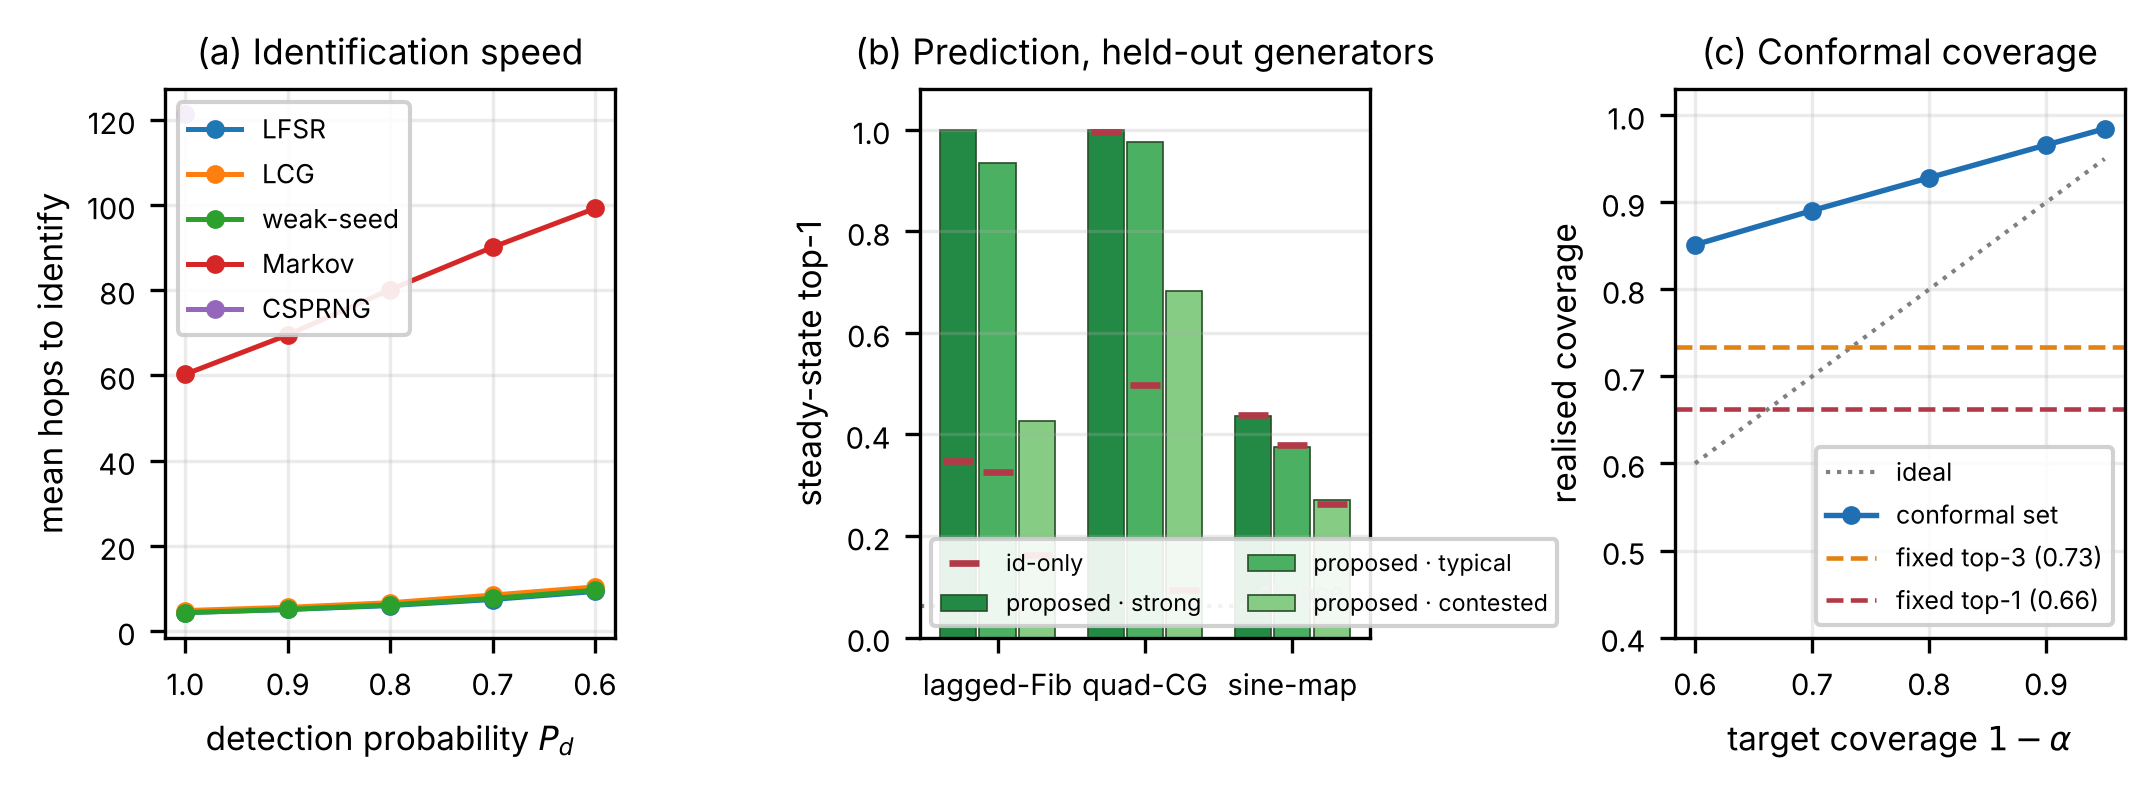
\includegraphics[width=0.98\textwidth]{fig_results.png}
\caption{(a) Mean hops-to-identify vs $P_d$: deterministic families need a
handful of hops, Markov an order of magnitude more. (b) Steady-state top-1
next-channel accuracy on the three held-out generators (bars: proposed, across
sensors; red ticks: identification-only bank); the dotted line is chance. (c)
Conformal coverage calibration: the set tracks the target, fixed shortlists do
not.}
\label{fig:results}
\end{figure*}

\begin{table}[t]
\centering
\caption{Steady-state top-1 next-channel accuracy, proposed predictor (P) vs
identification-only bank (I), across sensors (chance $=0.0625$, 30 seeds).}
\label{tab:predict}
\setlength{\tabcolsep}{3pt}
\footnotesize
\begin{tabular}{@{}lcccccc@{}}
\toprule
 & \multicolumn{2}{c}{Strong} & \multicolumn{2}{c}{Typical} & \multicolumn{2}{c}{Contested} \\
Generator & P & I & P & I & P & I \\
\midrule
LFSR (in-bank)          & 1.00 & 1.00 & 1.00 & 1.00 & 1.00 & 1.00 \\
lagged-Fib.\ (held out) & \textbf{1.00} & 0.35 & \textbf{0.94} & 0.33 & \textbf{0.43} & 0.16 \\
quad.-CG (held out)     & 1.00 & 1.00 & \textbf{0.98} & 0.50 & \textbf{0.68} & 0.09 \\
sine map (held out)     & 0.44 & 0.44 & 0.38 & 0.38 & 0.27 & 0.26 \\
CSPRNG (control)        & 0.07 & 0.07 & 0.07 & 0.06 & 0.06 & 0.06 \\
\bottomrule
\end{tabular}
\end{table}

\subsection{Switch tracking and the cost of identification}
Table~\ref{tab:switch} replays $24$ random switch plans over all thirteen
algorithms ($113$ switches) through the switch tracker. Switches are detected in
$95$--$97\%$ of cases with a median delay of $0$ hops on a perfect sensor and
$12$ on a contested one; dangerous locks stay at or below $0.015$ per regime
(two across the whole contested run). Finally, the measured
hops-to-identify sits within $1.3$--$2.7\times$ an information-theoretic lower
bound $\mathbb{E}[\tau]\geq\log((1-\delta)/\delta)/D$ with the posterior
log-odds drift $D$ estimated on the runs (mean efficiency $2.2\times$, always at
or above the floor), so the empirical stopping law is near-tight rather than
merely a good fit.

\begin{table}[t]
\centering
\caption{Switch tracking: 24 random plans over 13 algorithms (113 switches),
$M=16$.}
\label{tab:switch}
\setlength{\tabcolsep}{3pt}
\footnotesize
\begin{tabular}{@{}lcccc@{}}
\toprule
Sensor & Perfect & Strong & Typical & Contested \\
\midrule
Switches detected        & 97\% & 97\% & 97\% & 95\% \\
Delay, median/90th (hops)& 0/6  & 1/7  & 4/12 & 12/34 \\
Dangerous locks /regime  & .000 & .000 & .000 & .015 \\
Top-1, hops 6--10        & 0.72 & 0.65 & 0.53 & 0.20 \\
\bottomrule
\end{tabular}
\end{table}

%=======================================================================
\section{Discussion}
%=======================================================================
\emph{One likelihood explains the curves.} Every deterministic family is scored
by enumerating its parameters through \eqref{eq:emit}. This single choice
accounts for single-digit hops to identify, cost that scales as $1/P_d$, and
immunity to false alarms---a phantom scales every candidate equally and cancels.

\emph{Hard versus soft errors.} The dangerous error is a confident, false claim
of an algebraic break; it would send an operator after the wrong generator. That
rate is at most $0.05$ across every sensor and all coverage episodes, while a
closed-set test without $H_0$ makes it on every out-of-bank source. The case for
an explicit generative $H_0$ is this asymmetry, not raw accuracy.

\emph{A limited bank does not limit prediction as much.} Any bank is finite, and
an adversary can pick a generator outside it. Because the Fixed-Share mixture
weights experts by recent skill, the training-free universal expert takes over
within a few slots; the lagged-Fibonacci result ($1.00$ vs $0.35$) is the clear
case. Where a source is only statistically structured (sine map, Markov), the
mixture does no better than its best statistical learner---the honest limit.

\emph{Limitations.} All results are simulated with a slot-synchronous, i.i.d.\
sensor; hop-timing jitter, bursty fades and interleaved emitters are future
work. $M=16$ confounds the full-state LCG (period $\leq 16$) with a Markov
cycle. The generators and experts share authors, which the held-out families
mitigate but do not remove. The e-process guarantee is proven only for in-bank
truths; out-of-bank protection is empirical, via $H_0$.

%=======================================================================
\section{Conclusion}
%=======================================================================
OTS reduces a lossy passive sensor to one detection-level likelihood and reuses
it across a heterogeneous generator bank, a training-free next-channel
predictor, a change-point tracker and a conformal prediction set. The result is
a system that names in-bank generators quickly and safely, keeps predicting on
generators it was never built for, re-identifies a mid-engagement change of
algorithm, and attaches a distribution-free coverage guarantee to its forecast
that transfers to the response. Each component has a published ancestor; the
contribution is the sensor-aware assembly and its FH application. Future work
targets mis-specified and bursty sensors from real captures, larger channel
sets, and external learned baselines.

%=======================================================================
\begin{thebibliography}{00}
\bibitem{li2020lstm} G. Li \emph{et al.}, ``LSTM-based frequency hopping
sequence prediction,'' in \emph{Proc. WCSP}, 2020.
\bibitem{li2021china} G. Li \emph{et al.}, ``Frequency-hopping frequency
reconnaissance and prediction for non-cooperative communication network,''
\emph{China Commun.}, 2021.
\bibitem{zhu2023recovery} J. Zhu \emph{et al.}, ``Deep-learning-based recovery
of frequency-hopping sequences for anti-jamming applications,''
\emph{Electronics}, vol.~12, no.~3, 2023.
\bibitem{basak2024spectrum} S. Basak \emph{et al.}, ``Spectrum prediction for
protocol-aware RF jamming,'' \emph{IEEE Trans. Cogn. Commun. Netw.}, 2024.
\bibitem{strickland2023} C. Strickland \emph{et al.}, ``Predicting jamming
systems frequency hopping sequences using artificial neural networks,'' in
\emph{Proc. IEEE SoutheastCon}, 2023.
\bibitem{tao2025transformers} T. Tao, A. Doshi, V. Kalra, M. He, and
M. Barkeshli, ``(How) can transformers predict pseudo-random numbers?'' in
\emph{Proc. ICML}, 2025.
\bibitem{lee2020detection} K.-G. Lee \emph{et al.}, ``Detection of
frequency-hopping signals with deep learning,'' \emph{IEEE Commun. Lett.}, 2020.
\bibitem{baum1994} C. W. Baum and V. V. Veeravalli, ``A sequential procedure for
multihypothesis testing,'' \emph{IEEE Trans. Inf. Theory}, 1994.
\bibitem{dragalin1999} V. P. Dragalin, A. G. Tartakovsky, and V. V. Veeravalli,
``Multihypothesis sequential probability ratio tests,'' \emph{IEEE Trans. Inf.
Theory}, 1999.
\bibitem{ramdas2023} A. Ramdas \emph{et al.}, ``Game-theoretic statistics and
safe anytime-valid inference,'' \emph{Statist. Sci.}, vol.~38, no.~4, 2023.
\bibitem{gutman1989} M. Gutman, ``Asymptotically optimal classification for
multiple tests with empirically observed statistics,'' \emph{IEEE Trans. Inf.
Theory}, 1989.
\bibitem{barshalom2009} Y. Bar-Shalom, F. Daum, and J. Huang, ``The
probabilistic data association filter,'' \emph{IEEE Control Syst. Mag.}, 2009.
\bibitem{valyrakis2009} A. Valyrakis \emph{et al.}, ``Stochastic modeling and
particle filtering algorithms for tracking a frequency-hopped signal,''
\emph{IEEE Trans. Signal Process.}, 2009.
\bibitem{sidiropoulos2006} N. Sidiropoulos \emph{et al.}, ``Tracking a frequency
hopped signal using particle filtering,'' in \emph{Proc. IEEE ICASSP}, 2006.
\bibitem{knoblauch2018} J. Knoblauch and T. Damoulas, ``Spatio-temporal Bayesian
on-line changepoint detection with model selection,'' in \emph{Proc. ICML},
2018.
\bibitem{adams2007} R. P. Adams and D. J. C. MacKay, ``Bayesian online
changepoint detection,'' arXiv:0710.3742, 2007.
\bibitem{gibbs2021} I. Gibbs and E. Cand\`es, ``Adaptive conformal inference
under distribution shift,'' in \emph{Proc. NeurIPS}, 2021.
\bibitem{massey1969} J. L. Massey, ``Shift-register synthesis and BCH
decoding,'' \emph{IEEE Trans. Inf. Theory}, 1969.
\bibitem{reeds1977} J. Reeds, ``Cracking a random number generator,''
\emph{Cryptologia}, 1977.
\bibitem{blueear2016} W. Albazrqaoe, J. Huang, and G. Xing, ``Practical
Bluetooth traffic sniffing: systems and privacy implications,'' in
\emph{Proc. ACM MobiSys}, 2016.
\bibitem{qi2024drl} J. Qi \emph{et al.}, ``Deep reinforcement learning based
hopping strategy for wideband anti-jamming wireless communications,''
\emph{IEEE Trans. Veh. Technol.}, 2024.
\bibitem{herbster1998} M. Herbster and M. K. Warmuth, ``Tracking the best
expert,'' \emph{Mach. Learn.}, 1998.
\end{thebibliography}

\end{document}
